%---------------------------------------------
% Framework to Classify and Understand Research on Group Formation
%---------------------------------------------
\section{Study 1: Framework to Understand and Classify Research in CSCL}
\todo[inline]{FAZER O UPDATE E ESCREVER AQUI NOVOS  DADOS}

There are several denominations for the act of grouping learners in the context of collaborative learning, such as, group/team composition (Hsu et al. 2008) group or team formation (Yannibelli and Amandi 2012), grouping students (Alfonseca et al. 2006), clustering students (Chiu and Hsiao 2010). Basically, these denominations have the same meaning, as the act of bringing together students in effective learning groups (Isotani et al. 2009). In this work, we adopt the term group formation, which is the most widely term used in the investigated studies.

Although the term "effective" can have different meanings among researchers, in this field is often used as a synonym for the proper allocation of resources to enhance the learning process (Isotani et al. 2009). These resources can be tangible (e.g. learning materials and tools to support collaboration) or intangible (e.g. knowledge and skills to be learned). Most research on group formation have focused on how to allocate these resources based on the learners profiles, on the technologies involved, or on the tasks to be performed (CL techniques, also knows as CL best practices) (Magnisalis et al. 2011).
Using learners' profiles helps instructors adequately deliver custom content to satisfy, not only individual necessities of the learners, but also group's necessities (Alfonseca et al. 2006; Faria et al. 2006; Greer et al. 1998; Ounnas et al. 2009; Graf and Bekele 2006), while inputs from the environment, can give more information that can help to understand the collaborative context and as a result, to improve grouping quality (Muehlenbrock 2005; Villasclaras-Fernández et al. 2009; Hernández-Leo et al. 2011; Wesner and Pfister 2001) . Finally, there are other approaches for group formation that relies on using specifications of CL techniques to acquire sufficient information to group the learners (Isotani et al. 2009). 

Generally, the formation of groups can be performed randomly (e.g. assigning learners in the groups by chance), self-selected (i.e. the learners choose with whom they want to study), or it can be carried out by an instructor or computing system, based on some criteria (Ikeda and Mizoguchi 1997; Alfonseca et al 2006; Graf and Bekele 2006; Hsu and Chou 2008; Ounnas et al. 2009; Boticki et al. 2013; Greer et al. 1998; Faria et al. 2006)
As discussed by (Dillenbourg and Jermann 2007) and (Laurillard 2009), the benefits of collaborative learning arise only when there is a detailed and proper planning of components and collaborative mechanisms. Considering these, many authors have raised concerns regard random selection and self-selected approaches since these approaches can result in unequal participation such as, students in the same group working at a different pace, off-task behavior, or even increasing students’ resistance to group work (Barkley et al. 2005; Dillenbourg 2002; Isotani and Mizoguchi 2008; ). Moreover, one way to increase the chances of forming groups more capable to achieve the desired learning goals is assigning learners to groups using approaches based on CL techniques (Barkley et al. 2005; Dillenbourg 2002; Stahl 2004; Isotani et al. 2009).

Regardless of the strategy used, the research in the area sought to investigate ways to influence positively the behavior of individuals to form groups where their presence and that of their peers are relevant; that interactions are significant; and to maximize the chances that knowledge construction will occur in more favorable conditions. 
As discussed in the previous paragraphs, there are several topics being investigated under the umbrella of group formation research. Thus, to better understand the contribution of the community we propose a framework based on our understanding of the field. This framework (Figure 1) is composed of six main categories and their relationships: 

\begin{enumerate}
\item Planning: The formation of groups can either follow a set of criteria (i.e., systematic group formation) or happen randomly (i.e., unsystematic group formation). The criteria define the conditions that govern group formation, and the clustering algorithms determine how students should be selected and grouped together.
\item Initiative: to form groups we define two types of initiatives: spontaneous and controlled. Spontaneous group formation uses only the preferences of students to forming groups. This allows for the formation of like-minded groups of students. Controlled group formation, on the other hand, entails putting forward criteria and algorithms aimed at guiding the formation of groups. It might lead to heterogeneous groups in hopes of taking advantage of the resulting diversity of backgrounds as well as enhancing the overall learning experience. 
\item Diversity of population: Given each particular criterion, the population diversity in a group can be considered either homogeneous (i.e., whose participants have the same or similar trait) or heterogeneous to various degrees (i.e., participants differ from each other in at least one trait), depending on the amount of distinct individuals in the group regard the considered criterion. 
\item Distribution approach: Despite how many criteria a group formation strategy uses, if students end up distributed either in homogeneous or heterogeneous groups, we named the distribution approach as being Simple. However, when more than one criterion is used, the distribution of students can result in one (or more) criterion used to group the students homogeneously, while another different criterion (or criteria) being used to distribute the students heterogeneously. As a result, these groups can be considered homogeneous and heterogeneous at the same time, given the considered criterion. We named such distribution approach as Hybrid distribution.
\item Computer-supported: group formation can be very simple by using only one criterion (e.g. gender) or quite complex (using several criteria and algorithms). Thus, it is possible to categorize studies whose group formation approach relies on computational support and studies that report on approaches that do not rely on any sort of automated support for group formation.
\item Rationale: studies can also be classified in terms of how they back up their approach for group formation. In this framework we classify three types: studies that do not present any arguments that back up their approaches, studies whose group formation approach is borne out by empirical evidence, and studies that draw on assumptions from pedagogical theories.
\end{enumerate}

The categories are connected in the framework according to the following rationale: in general, the formation of groups is based on information (or lack of information) on the learner profiles. (1) The formation of groups can be planned or being randomly carried out. In the case of being planned, it can be based on grouping any criteria. Several criteria can be used, such as information about the students, students’ preferences, or even constraints of the system or environment. (2) When the students decide the clustering process, the initiative is spontaneous. When students do not participate in the selection process, and any other criterion is used to distribute them in groups, group formation is called controlled. (3) Criteria can be used both to group students with bases in their similarities (homogeneous groups) and/or in their differences (heterogeneous groups). (4) In simple distribution, the groups are mutually exclusive, being either homogeneous or heterogeneous; however, there are hybrid approaches in which groups are, at the same time, homogeneous and heterogeneous. (5) The formation of groups can be done manually, or it can rely, wholly or partially on computational systems. (6) Finally, the rationale provided in the studies allows us to understand whether the study is based on any pedagogical approach or based on empirical evidence; yet it is still possible to find studies which neither one nor another kind of justification for the formation of groups is provided.
    
\begin{figure}[h!]
\caption{Overview of the framework to classify and understand research on group formation..}
\centering
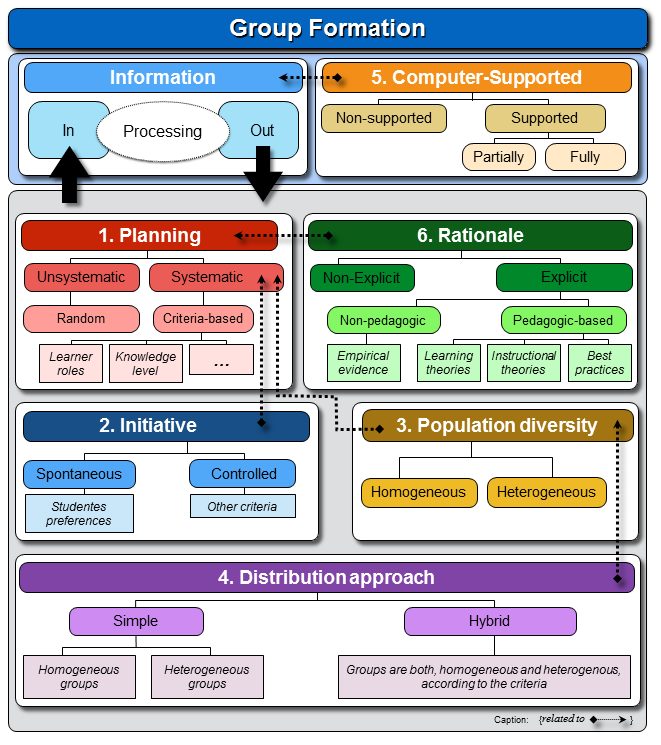
\includegraphics[]{gf_framework_full}
\end{figure}

Figure 1 gives an overview of our framework that can be used to classify, analyze and understand different types of research on the topic. The categories in the framework are tailored to give an overview of the efforts that have been carried out in the area, support the comprehension of the most investigated topics, and highlight the interacting and overlapping topics. Nevertheless, it is worth emphasizing the categories we came up with are not exhaustive. That is, they do not cover all the dimensions of the research spectrum of group formation in the context of CSCL. For example, the group activities were planned to occur face-to-face or in a distance learning way? The activities will occur synchronously or asynchronously?

In addition, we created three categories not showed in Figure 1. The purpose of these categories is to support gathering information about the way the selected researches have being conducted, and not directly about the group formation process.

\begin{itemize}
\item Educational level (or learning activities): By analyzing in which in educational contexts group formation has been explored, one can determine research gaps and future research opportunities;
\item Research methods: This category characterizes the type of research that has been carried out and reported in the studies;
\item Publication type: As for the publication types, we have selected primary studies that have been published in conferences, journals, and workshops.
\end{itemize}